\documentclass[a4paper,dvipdfm]{article}
%------------------------------------------------------------------------------------------------------
%\usepackage[symbol]{footmisc}这个宏包的作用是更改脚注的一些排版方式选项有: perpage stable side multiple para symbol ragged marginal flushmargin hang
%\usepackage{abstract}%这个红包的作用是双栏排版时,让摘要不这样,使用onecolabstract环境即可
\usepackage{booktabs}%for \toprule \midrule \bottomrule
\usepackage{fix2col}%修补在双栏排版时无法保证浮动体的排印顺序
\usepackage{fontspec,xltxtra,xunicode}    % 这里使用 xetex 相应的宏包
\usepackage{indentfirst} 					%缩进章节或者section里的第一段
\usepackage{url}
\usepackage{natbib} %cite URL
\usepackage{graphicx}
\usepackage{epsfig}
\usepackage[left=1.8cm,right=1.8cm,top=2cm,bottom=1.5cm]{geometry}
%\usepackage[left=0.1in, right=0.1in,  top=0.1in, bottom=0.1in, papersize={91.44mm, 121.92mm}]{geometry} %this is for kindle ebook
\usepackage{zhfont}                       % 这里调用 zhfont.sty 
%\usepackage[left=1.8cm,right=1.8cm,top=2cm,bottom=1.5cm]{geometry}
%\setzhmainfont{Microsoft JhengHei}
\setmainfont{Georgia}
\zhspacing

%以下是把论文中的一些参数中文化,比如摘要、参考文献等
\XeTeXlinebreaklocale “zh”
\XeTeXlinebreakskip = 0pt plus 1pt
\renewcommand\arraystretch{1.5}
\renewcommand{\contentsname}{目录}
\renewcommand{\listfigurename}{插图目录}
\renewcommand{\listtablename}{表格目录}
\renewcommand{\refname}{参考文献}
\renewcommand{\abstractname}{摘要}


\usepackage{tipa}
\usepackage{textcomp}





\pagestyle{empty}

\begin{document}
\title{WebKit总结}
\author{}
\maketitle
%put your book content here use \input{book.tex}
%{\setromanfont{Earwig Factory}\Huge\hfill Edit with \LaTeX  \tiny $_R^Y$}
\section{简介}
现在的WebKit项目起源于KDE项目的KHTML模块,苹果公司开发浏览器时对当时开源浏览器作了分析后决定采用KHTML模块,后根据协议将修改过的开源,命名为WebKit,有三个模块:
\begin{itemize}
	\item WebKit 与OS交互
	\item WebCore Render engine,是WebKit的核心
	\item JavaScriptCore JavaScript解析引擎
\end{itemize}

WebKit并不是浏览器,只是一个排版引擎,与\LaTeX 本质上类似,而排版内容和复杂度不可同日而语。针对不同的平台对WebKit的封装和绑定,官网称为port,比如比较流行的QtWebKit port和GTKWebKit port。本文旨在对WebKit内部及QT与GTK port中JavaScript引擎与WebKit交互及graphic system有个比较深入的了解。
\section{内部机制}
简单来讲,WebKit内部的工作机制分以下几个步骤:
\begin{enumerate}
	\item curl获得请求的stream数据
	\item DOM/Render树的创建
	\item JS/CSS操纵DOM
	\item Render
\end{enumerate}
\subsection{获取请求网页的数据}
网络处理部分提供ResourceHandle类供不同的平台库实现,具体可以在WebCore/platform/network里可见。//有时间继续,我们对此部分修改的可能性不大
\begin{itemize}
	\item 网络资源load机制
	\item Google SPDY它修改哪部分内容,强悍在哪里?
\end{itemize}
\subsection{DOM/Render树的创建}
\subsubsection{DOM/Render树根节点的创建}
HTMLDocument类中通过私有方法createParser()来创建DocumentParser,而DocumentParser中通过HTMLTreeBuilder和HTMLTokenizer来创建DOM树。如图\ref{fig:document_element}可见。
\begin{figure}[ht]
	\begin{center}
		\includegraphics[width=110mm]{image/dom-render-tree.ps}
	\end{center}
	\caption{DOM树创建重要变量}
	\label{fig:document_element}
\end{figure}
收到部分数据以后就开始了DOM树和Render树的创建。创建流程如图\ref{fig:dom_create}所示:
\begin{figure}[ht]
	\begin{center}
		\includegraphics[width=80mm]{image/dom-create.ps}
	\end{center}
	\caption{DOM Root creation}
	\label{fig:dom_create}
\end{figure}

由图\ref{fig:init_render_root}的流程开始了Render树根节点的创建,需要说明以下:
\begin{enumerate}
	\item 两棵树同时创建,Render树上只有DOM树上可见的元素,而诸如head等元素则不会出现在Render树中。同步创建的原因是为了更好的用户体验。所以为了尽可能快的呈现内容,不会去等DOM树生成好了再去创建Render树。
	\item HTML页面的根标签<html>不是DOM树的根节点,DOM树的根节点为HTMLDocument类型,而<html>标签所代表的类则是HTMLHtmlElement类,与此类似所有HTML页面中的标签都可以在WebCore/html/中找到相对应的类,HTML页面根标签<html>对应的节点为DOM树根节点的子节点。
\end{enumerate}
\begin{figure}[ht]
	\begin{center}
		\includegraphics[width=80mm]{image/call.ps}
	\end{center}
	\caption{RenderTree root creation}
	\label{fig:init_render_root}
\end{figure}
\subsubsection{DOM/Render节点的创建与添加}
以HTMLHtmlElement(<html>)节点的创建为例,它的创建过程如图\ref{fig:node_create}所示。
\begin{figure}[ht]
	\begin{center}
		\includegraphics[width=90mm]{image/node-create.ps}
	\end{center}
	\caption{DOM树非根节点的创建}
	\label{fig:node_create}
\end{figure}
\subsection{Layout}
\begin{enumerate}
	\item  Layout 和 Paint 这两个过程完全分开。开始执行Paint过程以前,必然预先执行过Layout,否则图形库就不知道在哪里写字以及显示图像。但是这并不意味 着,Layout执行结束后,随即就立刻执行Paint。实际上,Layout执行结束后,触发一个事件,这个事件启动Paint过程。但是Paint过 程也可以被其它事件触发,譬如屏幕内容的切换,以及把隐藏的浏览器窗口复原等等。
	\item Layout 涵盖了所有CSS规定的布局要素。包括页面边缘与内容之间的空白,文字对插入图像的避让(floating),单列与多列,上下层覆盖(z-index)等等。
	\item 图像,视频播放器插件,Applet等等,在 Layout 被称作 Replaced Render Object。这些 Replaced 元素的宽度和高度可以由CSS规定。如果CSS没有规定,就解析这些元素的数据流,譬如一个JPG照片的metadata里,规定了这幅照片原件的宽度和 高度。如果元素自己也没有规定宽度高度,就使用Webkit提供的缺省值。
	\item 文字的宽度根据页面的排版来确定。譬如一页中包含多列文字,则每列文字宽度相等。每列文字的宽度,乘以列数,加上列与列之间的夹缝,加上页面边缘空白等 等,应当等于页面总的宽度。假设页面总的宽度已知,边缘空白,和列与列之间的夹缝的宽度也已知,就可以反推文字的宽度。
	\item Render Tree中每个节点在屏幕上的显示,都呈长方形格局。前面第3点和第4点,描述了宽度的确定。而高度的确定,取决于这个中间节点的所有后代节点的高度的总 和。对于 Replaced 元素来说,它的高度相对比较容易确定,而文字段落的高度,需要根据字数,字型,以及字体大小计算得出。
	\item 在 Layout 过程中,反复出现以 Repaint 为开头的子过程,例如 repaintAfterLayoutIfNeeded()。这些子过程的意义在于,当确定了某个节点的高度和宽度以后,需要对其前辈节点,和左右兄弟节 点的位置,做适当调整。严格意义上来讲,这不是repaint,而是relayout。
	\item 相对于 Layout 过程,Paint 过程的逻辑要简单得多。Paint的过程,大致按照深度优先的顺序,遍历整棵RenderTree。也就是说,从最左边的叶子节点开始,从左向右逐个绘制 RenderTree所有可以显示的叶子节点。所谓“可以显示的叶子节点”,是因为CSS中可以规定,不显示某些叶子。
\end{enumerate}
总结:
\begin{enumerate}
	\item Layout 是一个计算量很繁重的过程。之所以繁重,主要体现在估算完每个RenderTree节点的宽度尤其是高度以后,需要相应调整这个节点的前辈节点以及左邻右舍兄弟节点的位置。对于文字段落而言,它的高度有赖于字数,字体和大小,所以估算不容易准确。
	\item 有没有可能把Layout 过程,与第一遍 Paint 过程合二为一? 只要遍历一次RenderTree的所有叶子节点,绘制图像并码字。Paint过程结束后,各个叶子节点对应的长方形的起始位置的(X,Y)坐标,以及宽 度和高度都自然迎刃而解。然后再由叶子节点开始,逐步确定RenderTree中,各个中间节点的起始位置和宽度高度。这样做的好处是,可以大大降低 Layout 过程的成本。
	\item  Layout 过程假设每个RenderTree 的节点都对应一个长方形屏幕区域。受限于这个规定,类似于Figure 2的效果,就显示不出来。有没有可能取消这个限制?SVG不仅提供了强大的绘图能力,而且也提供了强大的排版布局能力。能不能把CSS当着SVG格式的一 个子集来看待?
\end{enumerate}

\section{WebKit Qt port}
\subsection{编译}
之前需要安装QT以及设置QTDIR变量。编译Qt源码的步骤如下:
\begin{verbatim}
./configure -debug -nomake example
make
sudo make install 
\end{verbatim}
\begin{verbatim}
./Tools/Scripts/build-webkit --qt --debug
\end{verbatim}
\section{WebKit Chromium Port}
Chromium采用的也是WebKit引擎,不过把JavaScriptCore替换成自家的V8引擎,在官方网页的文档上提到,做一个绝对安全和永远不会crash掉浏览器几乎是不可能的,所以需要有一些架构来退其次的保证浏览器的安全和良好的用户体验,针对安全Chromium提出并实现了sandbox模型,针对用户体验Chromium采用多进程架构来尽可能的不让用户感觉到任何阻塞的行为。主要分Browser和Renderer两大进程,之间通过有名管道来实现通信(IPC机制)。
\subsection{FileAPI}
\begin{quotation}
	Chromium fileapi is so messsy with its multiple process architecture

	\begin{flushright}
		Chromium FileAPI author: Eric
	\end{flushright}
\end{quotation}

这是我在询问FileAPI实现细节时,Google 工程师给我的回答,所以用gdb跟踪一番,发现确实如此,render端负责将fileapi的调用从javascript侧调用到WebKit/WebCore/fileapi中定义的接口,其次,chrmoium在WebKit/WebKit/中加了一层胶水层用以封装WebKit中Fileapi接口的定义。然后交由FileDispatcher通过封装过的有名管道IPC发送到Browser端。继而在Browser端由FileDispatcherHost接收消息,然后分发至对应的接口处理。一个readDirectory接口具体跟踪如下:
\begin{verbatim}
webkitRequestFileSystem in JavaScript
V8进行操作,会判断是否是apicall,如果是,则通过V8机制调用WebKit接口。

third_party/WebKit/Source/WebCore/fileapi/DirectoryReader.cpp
DirectoryReader::readEntries

third_party/WebKit/Source/WebCore/fileapi/DOMFileSystemBase.cpp
DOMFileSystemBaseo:readDirectory

third_party/WebKit/Source/WebKit/chromium/src/AsyncFileSystemChromium.cpp
AsyncFileSystemChromium::readDirectory

content/common/file_system/webfilesystem_impl.cc
WebFileSystemImpl::readDirectory

content/common/file_system/file_system_dispatcher.cc
FileSystemDispatcher::ReadDirectory

============Render Process File System 部分调用结束===========

content/browser/file_system/file_system_dispatcher_host.cc
FileSystemDispatcherHost::OnReadDirectory

browser进程接收render进程filesystem IPC消息

webkit/fileapi/file_system_operation.cc
FileSystemOperation::ReadDirectory

webkit/fileapi/file_system_file_util_proxy.cc
FileSystemFileUtilProxy::RelayReadDirectory

============发往file_thread============

webkit/fileapi/obfuscated_file_util.cc
bfuscatedFileUtil::ReadDirectory

继续往下去会发现file system中保存的文件相对于OS fs来讲,位置在.config/chromium/Default/File System/,并且用的是自家的NoSQL数据库:leveldb 此外在chromium源码路径:base/file_util_posix.cc中定义了跟本地文件系统交互的地方,删除操作如removeRecursively可以断到这里查看详情。
\end{verbatim}
\subsection{DOM/Render树生成}
出于安全性、cookie、http request次数考虑,所有与网络与本地系统交互的地方统一交由Browser进程去做,这样WebKit中资源Load一块就被Chromium废掉了,相应的在./webkit中进行实现。资源Load完毕后将数据交给HTMLDocumentParser,然后HTMLDocumentParser将文本字符的解析交给HTMLDocumentTokenizer来负责,HTMLDocumentTokenizer解析出一个一个的标签(html文档时是以标签为单位),HTMLDocumentParser将标签交给,HTMLTreeBuilder来构建dom树。有几个基础元素:
\begin{itemize}
	\item FrameView 负责laying out rendering tree
	\item RenderView Render树的根节点
	\item RenderObject 可见对象,即render tree上的节点数据结构,在DOM上都有对应。
\end{itemize}

\subsection{图形系统分析}
TODO
\end{document}
